\section{Exception handling}
Exceptions are abnormal conditions during execution of a library
routine.  A typical example is a function to open a file.  The
case, that the named file does not exist, would then be an
exception.  Such an exception causes the orginal process to fail.
But it is also possible to think of exceptional conditions, where
the original request could still be completed successfully, if an
additional piece of information is supplied from the application
program during the exception processing.  An example of the later
is access to an encrypted file.  In that case, the open routine
will interrupt at some point, prompt the user for the encryption
password, and then will either resume operation normally, if the
password appears to be good, or abort, if the password was wrong.
This shows, why the "`throw/try/catch"' scheme of C++ is
considered to be inappropriate: after the execution of a
\cq{throw} statement has been completed, it is impossible to
resume operation in the block that triggered the error.  Rather,
all exception handling should be done by calling back into the
application program, with the failed library routine remaining
active.  It is then to the application to decide, if it can
provide the missing information, if it requests an abort of the
whole application, or if a specific application block should be
restarted or left to overcome the error situation.

In general, handling an exceptional condition requires three
steps:
\begin{description}
\item[error generation] where an object describing the error
    in general or in detail is generated.
\item[error delivery] where that object is forwarded to one or
    more routines of the application, that may know how to
    handle the error.
\item[error handling] where the application decides about what
    to do with the problem.
\end{description}
Besides these, we also need language constructs for defining,
which errenous conditions can occur.  In the Mjolner BETA system,
all these operations are unified into the `exception' pattern.
The do part of that pattern does a default error handling: abort
the current application.  A specialization of that pattern will
typically be a virtual pattern, whose purpose is to describe an
error in the `msg' variable of the exception `pattern'.  That is
the task of error generation.  In an application program, that
virtual error pattern may be bound to an application specific
error handler.  The virtual binding takes the task of error
delivery.

This concept is elegant.  It requires only one pattern to be used
for each error.  However, it contains the big backdraw, that
error delivery is static.  Each error is delivered to at most one
error handler by a virtual binding.  However, if a specific error
handler is not present, or not able to handle a certain
condition, the exception should be propagated to a less specific
handler.  An example is illustrated in figure \ref{exc-tree}.
Let's assume, we got an interactive application.  In some window,
the user may input a file name, that is then openend and read in.
The open process may fail due to an `AccessError' or
`NoSuchFileError', the read process may trigger a `ReadError'.  A
sophisticated application may provide different handlers for all
three cases.  However, many application will want to process all
these errors under the `FileError' label: a pop up box is posted
to the GUI, where an error message is printed, the errenous file
is closed, and a \cq{leave} imperative is executed for the
pattern, whose purpose is to open and read in the file.  So, if
an `AccessError' is not handled, it should be delivered to
`OpenError', then to `FileError' and finally to `StreamError'.

\begin{figure}[tbp]
\centerline{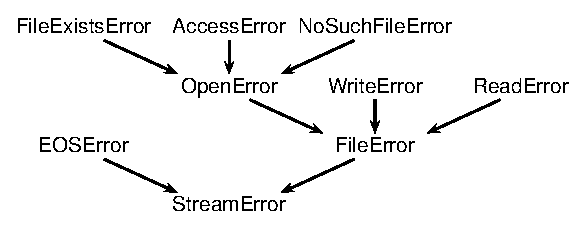
\psfig{file=extree.ps}}
\caption{Example of an exception tree structure.}
\label{exc-tree}
\end{figure}
The solution is to use two different patterns.  \cq{raise} is
used to raise an exception.  In its DO part, the \cq{deliverTo}
method can be used several times to deliver the error condition
to various exception handlers.  An exception handler is now a
direct subpattern of the \cq{exception} pattern, which is
specified as usual by a virtual binding declaration.

For the user of a library, this concept is fully backwards
compatible.  However, the writer of a library has to change the
code for raising an exception.  The exception pattern is written
such, that the old-style exception handling is still possible,
too.
